\documentclass[conference]{IEEEtran}
\IEEEoverridecommandlockouts
% The preceding line is only needed to identify funding in the first footnote. If that is unneeded, please comment it out.
\usepackage{cite}
\usepackage{amsmath,amssymb,amsfonts}
\usepackage{algorithmic}
\usepackage{graphicx}
\usepackage{textcomp}
\usepackage{xcolor}
\usepackage{placeins}
\usepackage[hidelinks]{hyperref}
\usepackage{float}
\def\BibTeX{{\rm B\kern-.05em{\sc i\kern-.025em b}\kern-.08em
    T\kern-.1667em\lower.7ex\hbox{E}\kern-.125emX}}
\begin{document}

\title{Classificador Ingênuo de Bayes}

\author{\IEEEauthorblockN{Arthur Abrahão Santos Barbosa}
\IEEEauthorblockA{\textit{Universidade Federal de Pernambuco} \\
\textit{Centro de Informática}\\
Pernambuco, Brasil \\
aasb2@cin.ufpe.br}
\and
\IEEEauthorblockN{Filipe Samuel da Silva}
\IEEEauthorblockA{\textit{Universidade Federal de Pernambuco} \\
\textit{Centro de Informática}\\
Pernambuco, Brasil \\
fss8@cin.ufpe.br}
\and
\IEEEauthorblockN{Nigel Mendes de Lima}
\IEEEauthorblockA{\textit{Universidade Federal de Pernambuco} \\
\textit{Centro de Informática}\\
Pernambuco, Brasil \\
nml@cin.ufpe.br}

}

\maketitle





\section{Objetivos}
\subsection{Objetivo Geral}
Através da análise de algumas informações referentes a um indivíduo, usando um classificador ingênuo de Bayes, prever se o mesmo irá se inscrever em um depósito a prazo. 
\subsection{Objetivos Específicos}
\begin{itemize}
\item Compreender a implementação do classificador ingênuo de Bayes
\item Demonstrar a Importância do Aprendizado de máquina e suas aplicações
\end{itemize}
\section{Justificativa}
Este projeto foi escolhido com base na maneira organizada e completa que o conjunto de dados  foi disponibilizado e por sua afinidade em aplicar-se os conceitos existentes, o banco de dados pode ser encontrando do site Machine Learning Repository, com o nome de "Bank Marketing Data Set"\cite{b1}.


Sua função é prover dados sobre a possibilidade de um cliente aderir ou não o serviço prestado pela agência com base em testes com múltiplas entradas de dados e com duas saídas possíveis, sim ou não. Seu público alvo são principalmente bancos, qualquer área de estudo sobre comportamento social e estudos sobre aprendizagem de máquina.

\section{Base de Dados}
Os dados são referentes a campanhas de marketing direto, por meio de telefonemas,muitas vezes repetindo o contato com um mesmo cliente, de uma uma instituição bancária portuguesa. O objetivo de sua classificação é prever de antemão se um cliente irá aderir ou não um depósito a prazo(identificado como a variável y).
O banco de dados completo está distribuído em quatro conjuntos sendo eles:

\begin{itemize}
\item bank-additional-full.csv com todos os exemplos (41188) e 20 entradas, ordenadas por data (de maio de 2008 a novembro de 2010), muito próximo aos dados analisados em [Moro et al., 2014 ]

\item bank-additional.csv com 10\% dos exemplos (4119), selecionados aleatoriamente de 1) e 20 entradas.

\item bank-full.csv com todos os exemplos e 17 entradas, ordenadas por data (versão mais antiga deste conjunto de dados com menos entradas).

\item bank.csv com 10\% dos exemplos e 17 entradas, selecionadas aleatoriamente a partir de 3 (versão mais antiga deste conjunto de dados com menos entradas).
\end{itemize}

Para o projeto será usado o item 3 (bank-full.csv) contendo 16 variáveis de entrada e uma de saída sendo elas (Nota: os exemplos de entrada abaixo estão todos em inglês, pois é assim que se encontra no banco de dados):


\subsection{16 Variáveis de entrada:}

\begin{itemize}
    \item age: (numerico).

    \item job: tipo de trabalho (categórico: 'admin.','blue-collar','entrepreneur','housemaid','management','retired','self-employed','services','student','technician','unemployed','unknown').

    \item marital: estado civil (categórico: 'divorced','married','single','unknown'; nota: 'divorced' significa divorciado ou viúvo).

    \item education: (categórico: 'basic.4y','basic.6y','basic.9y','high.school','illiterate','professional.course','university.degree','unknown').

    \item default: possui crédito inadimplente? (categórico: 'no','yes','unknown').

    \item balance (numérico).

    \item housing: possui crédito de habitação? (categórico: 'no','yes','unknown').

    \item loan: possui crédito pessoal? (categórico: 'no','yes','unknown').

    \item contact: tipo de comunicação do contato (categórico: 'cellular','telephone').

    \item day: dia do último contato  (numérico).

    \item duration: duração do último contato em segundos (numeric, nota importante, este atributo pode afetar muito a saída, por exemplo se a duração for ‘0’ então y = ‘no’, todavia a duração é desconhecida até que a chamada tenha terminado, nesse caso y é conhecido, sendo assim a entrada só será  incluída se realmente for necessária).

    \item month: último mês do contato (categórico: 'jan', 'feb', 'mar', ..., 'nov', 'dec').

    \item campaign: número de contatos realizados durante a campanha para este contato (numerico, inclui o último contato feito).
    
    \item pdays: número de dias que se passaram desde o último contato de uma campanha anterior para este cliente (numérico; 999 significa que este cliente não foi contatado antes).

    \item previous: número de contatos realizados para este cliente antes dessa campanha (numérico).

    \item poutcome: resultado da campanha de marketing anterior (categórico: 'failure','nonexistent','success').
\end{itemize}

\subsection{Uma Variavel de saida:}
\begin{itemize}
    \item y : o cliente assinou o depósito a prazo (binário: ‘yes’, ‘no’) .
\end{itemize}


\section{Análise Exploratória dos Dados}
\subsection{Descrição Estatística dos dados}
\begin{itemize}
	\item	O campo \textbf{\textit{count}}, representa a quantidade de instancias que contém aquele atributo.
	\item	O campo \textbf{\textit{unique}} se refere a quantas categorias existem daquele atributo, caso ele seja do tipo texto descritivo (não numérico).
	\item	O campo \textbf{\textit{top}} se refere a categoria mais encontrada daquele atributo.
	\item	O campo \textbf{\textit{freq}} é o número de vezes que a categoria top daquele atributo foi encontrada.
	\item	O campo \textbf{\textit{mean}} informa a média dos valores daquele atributo, caso sejam numéricos.
	\item	O campo \textbf{\textit{std}} informa o desvio padrão dos dados daquele atributo.
	\item	O campo \textbf{\textit{min}} mostra o menor valor numérico que aquele atributo possui nas amostras, considerando todas as instâncias.
	\item	O campo \textbf{\textit{25\%}} se refere ao primeiro quartil das amostras daquele atributo.
	\item	O campo \textbf{\textit{50\%}} se refere ao segundo quartil das amostras daquele atributo.
	\item	O campo \textbf{\textit{75\%}} se refere ao terceiro quartil das amostras daquele atributo.
	\item	O campo \textbf{\textit{max}} informa o maior valor que aquele atributo possui entre todas as amostras.
\end{itemize}
\subsection{Dados Disponíveis ou ausentes}
\begin{itemize}
	\item 	Os atributos \textbf{age, day, duration, campaign, pdays, previous}, possuem informação do tipo numérico e são valores quantitativos discretos.
	\item 	O atributo \textbf{balance}, possuui informação do tipo numérico e são valores quantitativos contínuos.
	\item 	Os atributos \textbf{job, marital, education, default, housing, loan, contact, poutcome}, possuem informação do tipo texto descritivo(categorias), seus valores são qualitativos nominais.
	\item 	Os atributo \textbf{month}, possui informação do tipo texto descritivo(categorias), seus valores são qualitativos ordinais.
	\item Não existem dados faltando(ausentes) em nenhum campo de nenhuma instância.
\end{itemize}
\subsection{Gráficos}
\begin{itemize}
	\item[(1)] 	Primeiro temos o Histograma (Fig.\ref{figura:distidade}) das idades em relação ao total de amostras.
	\subitem- 	Com destaque para a maior parte dos valores estarem próximos ao intervalo  entre 30 e 40 anos.
	\subitem- 	Temos a média como 40,936210, e o desvio padrão de 10,618762.
	\item[(2)] Segundo temos o número de pessoas que obtiveram emprestimo de casa em relação a sua grau de educação escolar (Fig.\ref{figura:fig2}).
	\subitem- 	Destaque para o grau secundário que tem a maior parte dos que pegaram empréstimo.
	\subitem-		O grau secundário(ensino médio) é o que mais aparece nas amostras.
	\item[(3)] Temos o grau da educação escolar em relação ao Saldo médio anual (Fig.\ref{figura:fig3}) 
	\subitem-		O destaque fica para os valores Outliers do saldo, principalmente pro grau tertiary(Faculdade).
	\begin{figure}[h]
		\caption{Exemplo}
		\centering % para centralizarmos a figura
		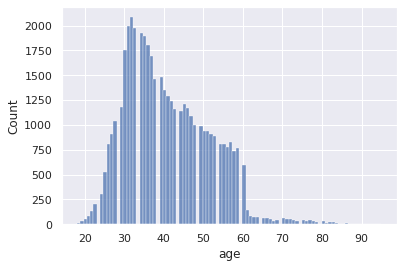
\includegraphics[width=8cm]{IMGS/img1.png}
		\label{figura:distidade}
		\caption{Exemplo2}
		%\centering % para centralizarmos a figura
		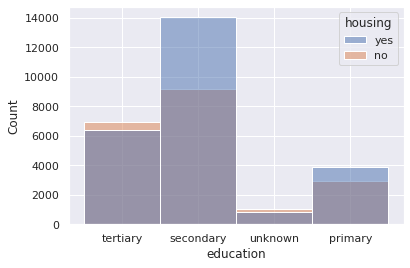
\includegraphics[width=8cm]{IMGS/img2.png}
		\label{figura:fig2}
		\caption{Exemplo4}
		\centering % para centralizarmos a figura
		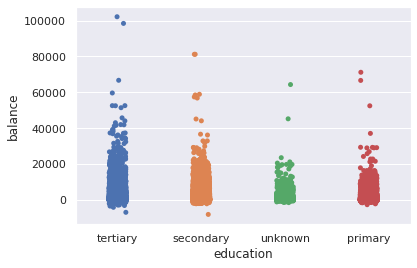
\includegraphics[width=8cm]{IMGS/img3.png}
		\label{figura:fig3}
	\end{figure}
	\item[(4)] Temos o número de empréstimos de casa em relação ao tipo de contato que foi registrado (Fig. \ref{figura:fig4}).
	\subitem-		O destaque está no tipo de contato cellular, que possui um número de emprestimo 'sim' muito próximo ao 'não', apesar de 25130 de todas as amostras serem com valor \textbf{\textit{sim}}.
	\item[(5)] Temos o boxplot (Fig.\ref{figura:fig5}) de empréstimo pessoal em relação a idade.
	\subitem-		Temos os valores do primeiro quartil, do terceiro quartil e da mediana de cada boxplot, para as respostas \textbf{\textit{sim}} e \textbf{\textit{não}}.
	\subitem-		Podemos ver que a mediana de ambos os boxplots, têm uma valores muito próximos.
	\subitem- 		Outro destaque vai para os outliers das amostras com respostas \textbf{\textit{sim}}.
	\begin{figure}[h]
		\caption{Exemplo4}
		\centering % para centralizarmos a figura
		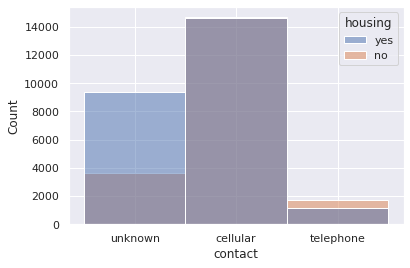
\includegraphics[width=8cm]{IMGS/img4.png}
		\label{figura:fig4}
		\caption{Exemplo5}
		%\centering % para centralizarmos a figura
		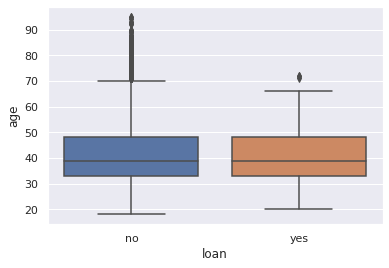
\includegraphics[width=8cm]{IMGS/img5.png}
		\label{figura:fig5}
	\end{figure}
	\item[(6)] Temos o strippplot (Fig.\ref{figura:fig6}) de empréstimo pessoal em relação a idade.
	\subitem-		Com destaque para as idades que foram os outliers, em relação ao Não Empréstimo, temos os mais velhos.
	\subitem-		Já do outro lado, os que sim, tiveram emprétimo pessoal estavam em um intervalo de idade menor, e mais jovem.
	\item[(7)] Temos o strippplot (Fig.\ref{figura:fig7}) dos meses em relação a campanha que foi realizada.
	\subitem-		Com destaque para os meses do meio do ano que contemplam a maior parte das amostras.
	\subitem-		Enquanto que no final do ano, foram registrados as menores parcelas das amostras.
	\begin{figure}[h]
		\caption{Exemplo6}
		\centering % para centralizarmos a figura
		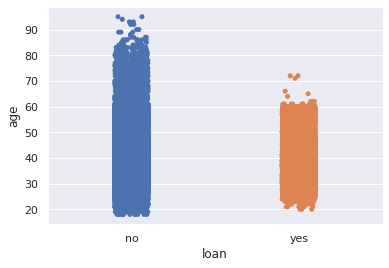
\includegraphics[width=8cm]{IMGS/img6.png}
		\label{figura:fig6}
		\caption{Exemplo7}
		%\centering % para centralizarmos a figura
		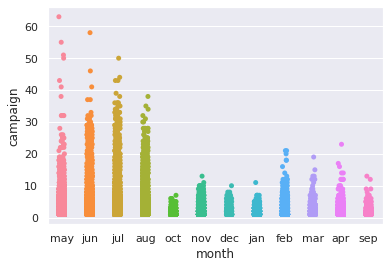
\includegraphics[width=8cm]{IMGS/img7.png}
		\label{figura:fig7}
	\end{figure}
\end{itemize}
\subsection{Outliers}
Nesta seção temos a quantidade de pessoas que aceitaram ou recusaram assinar um investimento, em cada classe ou categoria de cada atributo para os atributos do tipo texto descritivo, e em relação aos valores númericos de um atributo, para um atributo do tipo numérico. 
%\begin{itemize}
%	\item 
%\end{itemize}


\section{Classificador Ingênuo de Bayes}
Baseado no Teorema de Bayes, nome em homenagem ao matemático e pastor presibiteriano inglês Thomas Bayes, que formulou uma função probabilística com o ideal de provar a existência de Deus, Naive Bayes é um algoritmo de classificação probabilística muito utilizado para aprendizado de máquina (Machine Learning). O algoritmo possui a habilidade de categorizar textos baseado na frequência em que as palavras são dispostas, o exemplo mais comum são os filtros de e-mail que podem utilizar o Naive Bayes para identificar se uma mensagem é um spam apenas lendo a disposição das palavras utilizadas. O nome Naive, do português ingênuo, vem do fato que o algoritmo desconsidera totalmente a correlação entre as variáveis, tratando cada uma de maneira independente.

\subsection{Definição Formal do Teorema de Bayes}
O teorema é um corolário da lei da probabilidade total e é descrito da seguinte maneira, sejam A e B dois eventos e P(A) e P(B) as probabilidades de A e B, respectivamente, sendo P(B) diferente de 0, então o Teorema de Bayes nos diz que,

\begin{equation}
    P(A|B) = \frac{P(B|A)P(A)}{P(B)},
\end{equation} 
De maneira análoga, com P(A) diferente de 0,  
\begin{equation}
   P(B|A) = \frac{P(A|B)P(B)}{P(A)}.
\end{equation} 

\subsection{Tipos de Classificadores Ingênuos de Bayes}
A biblioteca Scikit learn apresenta diversos tipos de Classificadores. As diferenças principais entre eles são principalmente em relação as suposições feitas em relação a distribuição de probabilidade $P(x_i|y)$. 
No projeto foram-se aplicados dois tipos de Classificadores, o Gaussiano e o Categórico:

\subsubsection{Bayes Ingênuo Gaussiano}
O classificador de bayes gaussiano supõe que as variáveis seguem uma distribuição normal, a verossimilhança das variáveis são supostas como gaussianas:

\begin{equation}
    P(x_i|y) = \frac{1}{\sqrt{2\pi\sigma_y^2}}e^{-\frac{(x_i - \mu_y)^2}{2\sigma_y^2}}
\end{equation}

Os parametros $\sigma_y$ e $\mu_y$ são estimados usando máxima verossimilhança.

\cite{b5}
\subsubsection{Bayes Ingênuo Categórico}
O Bayes Ingênuo Categórico implementa o classificador de bayes ingênuo para distribuição categórica de dados.

A probabilidade de $x_i$ ser da categoria t dado a classe é c é estimado como:

\begin{equation}
    P(x_i = t | y = x; \alpha) = \frac{N_{tic} + \alpha}{N_c + \alpha n_i}
\end{equation}

onde:

\begin{itemize}
\item $N_{tic}$ é o número de vezes que a categoria t aparece na amostra e pertence a classe c
\item $N_c$ é o número de amostras que pertence a classe c
\item $\alpha$ é um parâmetro de calibração
\end{itemize}

\cite{b5}
\subsection{Sobre o Projeto}
Para montar o classificador foi necessário passar  pelas seguintes etapas:

\begin{figure}[H]
    \centerline{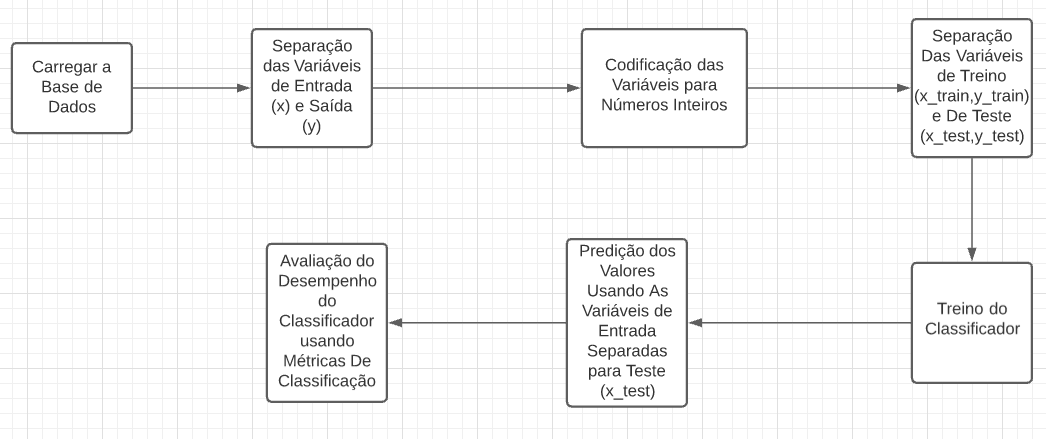
\includegraphics[width=0.4\textwidth]{IMGS/block1.png}}
    
    \caption{\label{fig:block1}Passo a Passo para Montar o Classificador Ingênuo de Bayes}
\end{figure}

\begin{enumerate}
\item Carregar o data frame através da biblioteca Pandas
\item Separação dos valores de x (entrada) e de y (saída)
\item Conversão dos valores da Base de Dados para números inteiros através do módulo preprocessing da biblioteca sklearn.model\_selection
\item Separação dos Dados para treino e para teste através do módulo train\_test\_split da biblioteca sklearn.model\_selection
\item Treino do Classificador Ingênuo de Bayes através dos módulos GaussianNB e CategoricalNB da biblioteca sklearn.naive\_bayes. Foram criados dois classificadores: Um Gaussiano que assume que todas as variáveis de treino são normais (o que não é verdade), e um categórico que assume que as variáveis de treino seguem uma distribuição categórica (Mais próximo da realidade).
\item Predição dos valores de usando as variáveis de entrada separadas para teste
\item Avaliação Do classificador Usando métricas de classificação
\end{enumerate}

\section{Experimentos}

\subsection{Experimentos Iniciais}
Após treinar ambos os classificadores (Gaussiano e Categórico), usando 20 por cento dos dados para teste. Foi verificado alguns valores referente ao teste:

\begin{itemize}
\item Precision: Precision é a razão
    \begin{equation}
        \frac{t_p}{t_p + f_p}
    \end{equation}

    onde:

    \begin{itemize}
    \item $t_p$ é o número de verdadeiros positivos
    \item $f_p$ é o número de falsos positivos.
    \end{itemize}

    Precision é intuitivamente a habilidade do classificador não marcar como positivo uma amostra que é negativa. O melhor valor de Precision é 1 e o pior é zero.
    \cite{b7}
\item Accuracy: accuracy é a fração de amostras preditas corretamente, e é dada pela seguinte fórmula:
\begin{equation}
    \frac{t_p + t_n}{t_p + t_n + f_p + f_n}
\end{equation}
onde:
\begin{itemize}
    \item $t_p$ é o número de verdadeiros positivos
    \item $f_p$ é o número de falsos positivos.
    \item $t_n$ é o número de verdadeiros negativos.
    \item $f_n$ é o número de falsos negativos.
\end{itemize}
\cite{b8}
\item Recall-Score: O Recall Score é a razão:
    \begin{equation}
        \frac{t_p}{t_p + f_n}
    \end{equation}
    onde:
    \begin{itemize}
    \item $t_p$ é o número de verdadeiros positivos
    \item $f_n$ é o número de falsos negativos
    \end{itemize}
    O Recall Score é intuitivamente a habilidade do classificador de encontrar todas as amostras positivas. O melhor valor do Recall Score é 1 e o pior valor é 0.
    \cite{b6}
\item F1-Score: O F1 Score pode ser interpretado como a média ponderada da precisão e recall. O melhor valor que o  F1 score pode alcançar é 1, o pior é 0. A contribuição relativa da precisão e recall para o F1 score são iguais. A fórmula para o F1 score é:
\begin{equation}
    F1 = \frac{2\cdot(precision\cdot recall)}{precision + recall}
\end{equation}
\cite{b2}
\item Confusion Matrix:
No caso de classificação binária uma confusion matrix é dividida em quatro categorias, cada uma apresentando a quantidade de valores que se encaixam nesta. Elas são:
\begin{itemize}
\item Verdadeiro Negativo: Valor Real = 0, Valor Predito = 0
\item Falso Negativo: Valor Real = 1, Valor Predito = 0
\item Falso Positivo: Valor Real = 0, Valor Predito = 1
\item Verdadeiro Positivo: Valor Real = 1, Valor Predito = 1
\cite{b8}
\end{itemize}
\end{itemize}
\begin{table}[H]
	\centering
    \caption{\label{tab:cr1-gt} Comparação entre o Classificador Categórico e o Gaussiano}
    \begin{small}
        \begin{tabular}{ccc}
        	\\
        	%\multicolumn{2}{c}{{\fontsize{13}{\baselineskip} \selectfont C}{\fontsize{11}{\baselineskip}\selectfont RONOGRAMA DE}{\fontsize{13}{\baselineskip} \selectfont A}{\fontsize{11}{\baselineskip}\selectfont TIVIDADES }}\\ 
        	\\
            \hline
                                    & Categórico       & Gaussiano\\
            \hline
            Precision               & 0.89             & 0.84\\
            Accuracy                & 0.89             & 0.84\\
            Recall Score            & 0.89             & 0.84\\
            F1-Score                & 0.89             & 0.84\\
            
            \hline
        \end{tabular}
    \end{small}
\end{table}

\begin{table}[H]

	\centering
    \caption{\label{tab:cr1-cnb} Relatório de Classificação por Label do Classificador Categórico.}
    \begin{small}
        \begin{tabular}{ccc}
        
            \hline
                                    & 0                & 1\\
            \hline
            Precision               & 0.93             & 0.53\\
            Recall Score            & 0.95             & 0.43\\
            F1-Score                & 0.94             & 0.47\\
            
            \hline
        \end{tabular}
    \end{small}

\end{table}

\begin{figure}[H]
\centerline{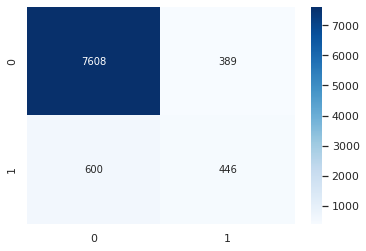
\includegraphics[width=0.4\textwidth]{IMGS/cm-categorico.png}}

\caption{\label{fig:cm1-cnb}Confusion Matrix do Classificador Categórico}
\end{figure}




\begin{table}[H]

	\centering
    \caption{\label{tab:cr1-gnb} Relatório de Classificação por Label do Classificador Gaussiano}
    \begin{small}
        \begin{tabular}{ccc}
        
            \hline
                                    & 0                & 1\\
            \hline
            Precision                & 0.89             & 0.49\\
            Recall Score            & 1.00             & 0.03\\
            F1-Score                & 0.94             & 0.06\\
            
            \hline
        \end{tabular}
    \end{small}

\end{table}


\begin{figure}[H]
\centerline{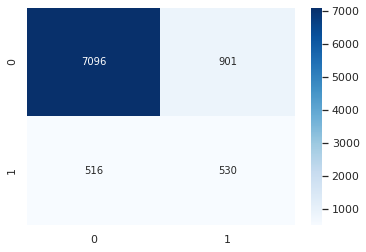
\includegraphics[width=0.4\textwidth]{IMGS/cm-gaussiano.png}}
\label{cm1-gnb}
\caption{\label{fig:cm1-gnb}Confusion Matrix do Classificador Gaussiano}
\end{figure}

\subsection{Usando Apenas a Variável Age Para Treino}
Foram usados 70 por cento dos valores para treino e 30 por cento dos valores para teste.

\begin{table}[H]
	\centering
    \caption{\label{tab:cr2-gt} Comparação entre o Classificador Categórico e o Gaussiano}
    \begin{small}
        \begin{tabular}{ccc}
        	\\
        	%\multicolumn{2}{c}{{\fontsize{13}{\baselineskip} \selectfont C}{\fontsize{11}{\baselineskip}\selectfont RONOGRAMA DE}{\fontsize{13}{\baselineskip} \selectfont A}{\fontsize{11}{\baselineskip}\selectfont TIVIDADES }}\\ 
        	\\
            \hline
                                    & Categórico       & Gaussiano\\
            \hline
            Precision               & 0.88             & 0.88\\
            Accuracy                & 0.88             & 0.88\\
            Recall Score            & 0.88             & 0.88\\
            F1-Score                & 0.88             & 0.88\\
            
            \hline
        \end{tabular}
    \end{small}
\end{table}


\begin{table}[H]

	\centering
    \caption{\label{tab:cr2-cnb} Relatório de Classificação por Label do Classificador Categórico.}
    \begin{small}
        \begin{tabular}{ccc}
        
            \hline
                                    & 0                & 1\\
            \hline
            Precision               & 0.88             & 0.50\\
            Recall Score            & 1.00             & 0.02\\
            F1-Score                & 0.94             & 0.04\\
            
            \hline
        \end{tabular}
    \end{small}
\end{table}

\begin{figure}[H]
    \centerline{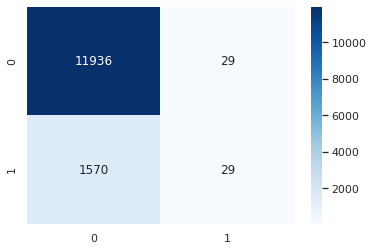
\includegraphics[width=0.4\textwidth]{IMGS/cm-cnb-age-only.png}}
    
    \caption{\label{fig:cm2-cnb}Confusion Matrix do Classificador Categórico}
\end{figure}


\begin{table}[H]

	\centering
    \caption{\label{tab:cr2-gnb} Relatório de Classificação por Label do Classificador Gaussiano}
    \begin{small}
        \begin{tabular}{ccc}
        
            \hline
                                    & 0                & 1\\
            \hline
            Precision               & 0.88             & 0.48\\
            Recall Score            & 1.00             & 0.03\\
            F1-Score                & 0.94             & 0.05\\
            
            \hline
        \end{tabular}
    \end{small}

\end{table}


\begin{figure}[H]
    \centerline{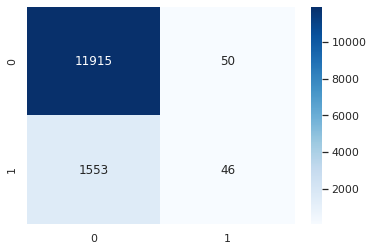
\includegraphics[width=0.4\textwidth]{IMGS/cm-gnb-age-only.png}}
    \caption{\label{fig:cm2-gnb}Confusion Matrix do Classificador Gaussiano}
\end{figure}

\subsection{Usando Apenas Variáveis Numéricas Para Treino}

\begin{table}[H]
	\centering
    \caption{\label{tab:cr3-gt} Comparação entre o Classificador Categórico e o Gaussiano}
    \begin{small}
        \begin{tabular}{ccc}
        	\\
        	%\multicolumn{2}{c}{{\fontsize{13}{\baselineskip} \selectfont C}{\fontsize{11}{\baselineskip}\selectfont RONOGRAMA DE}{\fontsize{13}{\baselineskip} \selectfont A}{\fontsize{11}{\baselineskip}\selectfont TIVIDADES }}\\ 
        	\\
            \hline
                                    & Categórico       & Gaussiano\\
            \hline
            Precision               & 0.89             & 0.89\\
            Accuracy                & 0.89             & 0.89\\
            Recall Score            & 0.89             & 0.89\\
            F1-Score                & 0.89             & 0.89\\
            
            \hline
        \end{tabular}
    \end{small}
\end{table}

\begin{table}[H]

	\centering
    \caption{\label{tab:cr3-cnb} Relatório de Classificação por Label do Classificador Categórico.}
    \begin{small}
        \begin{tabular}{ccc}
        
            \hline
                                    & 0                & 1\\
            \hline
            Precision               & 0.89             & 0.63\\
            Recall Score            & 0.99             & 0.11\\
            F1-Score                & 0.94             & 0.18\\
            
            \hline
        \end{tabular}
    \end{small}
\end{table}

\begin{figure}[H]
    \centerline{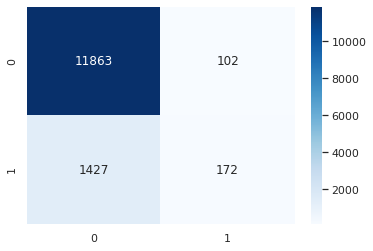
\includegraphics[width=0.4\textwidth]{IMGS/cm-cnb-numeric.png}}
    
    \caption{\label{fig:cm3-cnb}Confusion Matrix do Classificador Categórico}
\end{figure}


\begin{table}[H]

	\centering
    \caption{\label{tab:cr3-gnb} Relatório de Classificação por Label do Classificador Gaussiano}
    \begin{small}
        \begin{tabular}{ccc}
        
            \hline
                                    & 0                & 1\\
            \hline
            Precision               & 0.91             & 0.53\\
            Recall Score            & 0.96             & 0.32\\
            F1-Score                & 0.94             & 0.40\\
            
            \hline
        \end{tabular}
    \end{small}

\end{table}


\begin{figure}[H]
    \centerline{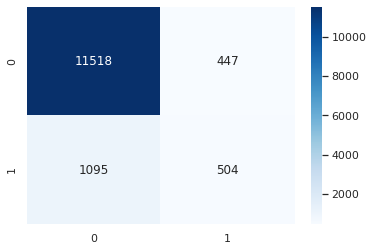
\includegraphics[width=0.4\textwidth]{IMGS/cm-gnb-numeric.png}}
    \caption{\label{fig:cm3-gnb}Confusion Matrix do Classificador Gaussiano}
\end{figure}


\section{Análise dos Resultados}

Como é possível ver através dos dados acima, Os três primeiros experimentos apresentam os valores de Precision, Accuracy, Recall e F1-Score
extremamente altos (acima de 80 por cento) porém ao análisar os resultados por label. verifica-se que há uma quantidade bem maior de verdadeiros negativos do que verdadeiros positivos.
Isso se evidencia ainda mais quando é usada apenas feature age para treinar o classificador, pois a quantidade de verdadeiros positivos diminui drásticamente.
Uma hipótese do motivo pelo qual acontece o ocorrido é que a base de dados tem mais exemplos de quando a variável y tem o valor no (mapeado para o label 0),
do que quando esta possui o valor yes (mapeada para o label 1).

Além disso pode-se observar que o Classificador Ingênuo de Bayes Categórico tem praticamente o mesmo desempenho do que o Classificador ingênuo de Bayes Gaussiano, o que não é o esperado pois boa parte das variáveis que a base de dados possui é do tipo categórico.


\section{Conclusões e Discussões}
O naive Bayes se apresenta como uma ótima ferramenta, de maneira simples e rápida, com um pequeno número de dados é possível identificar padrões de comportamentos com boa precisão, além do mais é possível, ao mesmo tempo, lidar com diferentes tipos de dados como real, discreto e contínuo, por exemplo, e descartar características irrelevantes.


Ao decorrer da análise pode ser que ocorra erros ao usar o Naive Bayes quando a probabilidade de algum atributo for 0, ou também chamado de frequência zero, produzindo uma previsão completamente falha, neste caso é necessário usar de técnicas de suavização como, por exemplo, a correção Laplaciana.Outra desvantagem é a de ignorar a correlação entre as variáveis, que até certo ponto de vista pode ser tido como vantagem, na realidade é muito improvável encontrar um conjunto de variáveis que sejam totalmente independentes.




\bibliography{mybib}
\nocite{*}
\bibliographystyle{IEEEtran}
\end{document}
